\section{Competition simulation and attribution}
\label{sec:competition}

We simulate \#1292 over the competition dates. The account stays in cash until
month-end.
Formation/execution dates are February 27/March 2, March 31/April 1 and
April 30/May 1, with ten longs and ten shorts in each invested interval.
Sizing uses the preceding close; overnight moves, integer shares and retained
positions explain deviations from the formation weights.

The account ends at \$1,538,521: a 53.85\% net return against 8.04\% for the
benchmark, or 45.82 percentage points of excess return. The gain follows a
March decline and sharp recovery in April and early May.

\begin{figure}[H]
  \centering
  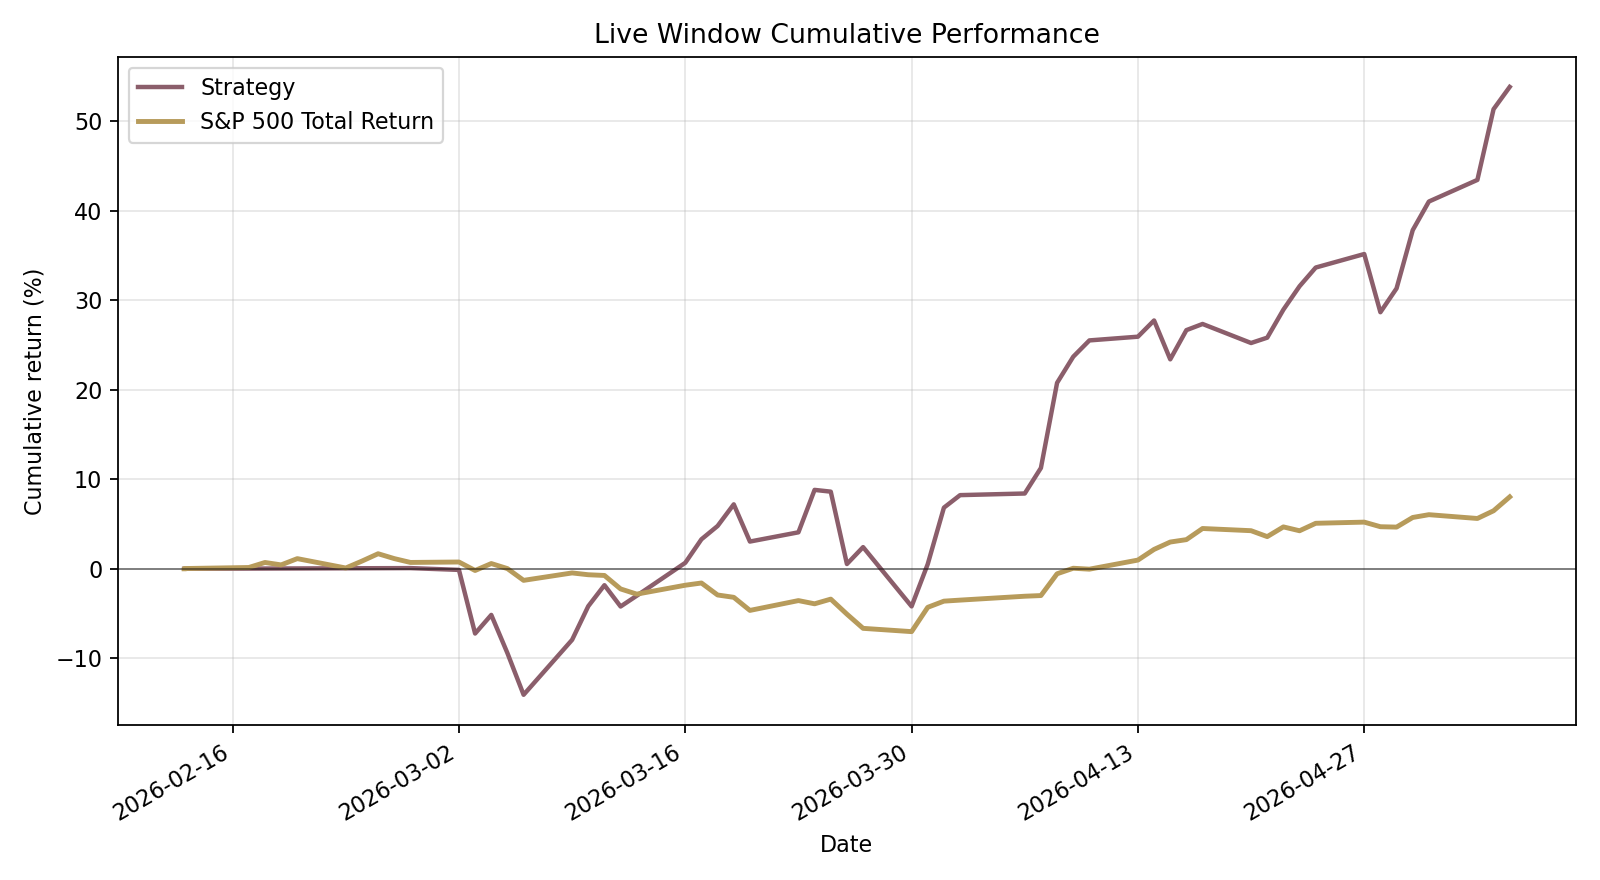
\includegraphics[width=\reportfigurewidth]{../outputs/live/strategies/momentum/figures/live_window/cumulative_performance.png}
  \caption[Competition-window cumulative net performance]{Net momentum simulation and S\&P 500 Total Return benchmark,
  February 13 open-May 6 close, 2026, including the initial cash phase.}
  \label{fig:competition-performance}
\end{figure}

\subsection{Risk and costs}

Risk statistics use 56 close-to-close returns, including the cash phase, at
252 observations per year. The initial open-to-close move enters cumulative
performance only. Risk-free accrual uses the 2\% Actual/365 rate; metric
formulas are in \cref{sec:performance-metrics}.

\begin{table}[H]
  \centering
  \begin{threeparttable}
  \small
  \begin{tabularx}{0.92\linewidth}{@{}X S[table-format=-3.2] S[table-format=-3.2]@{}}
    \toprule
    Metric & {Momentum} & {S\&P 500 TR} \\
    \midrule
    Annualized volatility (\%) & 52.28 & 15.11 \\
    Sharpe ratio & 3.94 & 2.24 \\
    Market beta & 1.99 & 1.00 \\
    Treynor ratio & 1.04 & 0.34 \\
    Information Ratio & 3.80 & {-} \\
    Tracking error (\%) & 45.33 & {-} \\
    Annualized CAPM alpha (\%) & 138.98 & 0.00 \\
    \bottomrule
  \end{tabularx}
  \caption[Competition-period risk metrics]{Competition-period risk metrics. Rates are annualized.}
  \label{tab:competition-risk}
  \end{threeparttable}
\end{table}

Beta near two indicates substantial market exposure. Annualizing the 53.85\%
gain over 82 calendar days gives 580.52\%. Annualized CAPM alpha was 138.98\%
($p=0.139$), not statistically significant at the 5\% level. The short sample
also limits the reliability of risk ratios.

\begin{figure}[H]
  \centering
  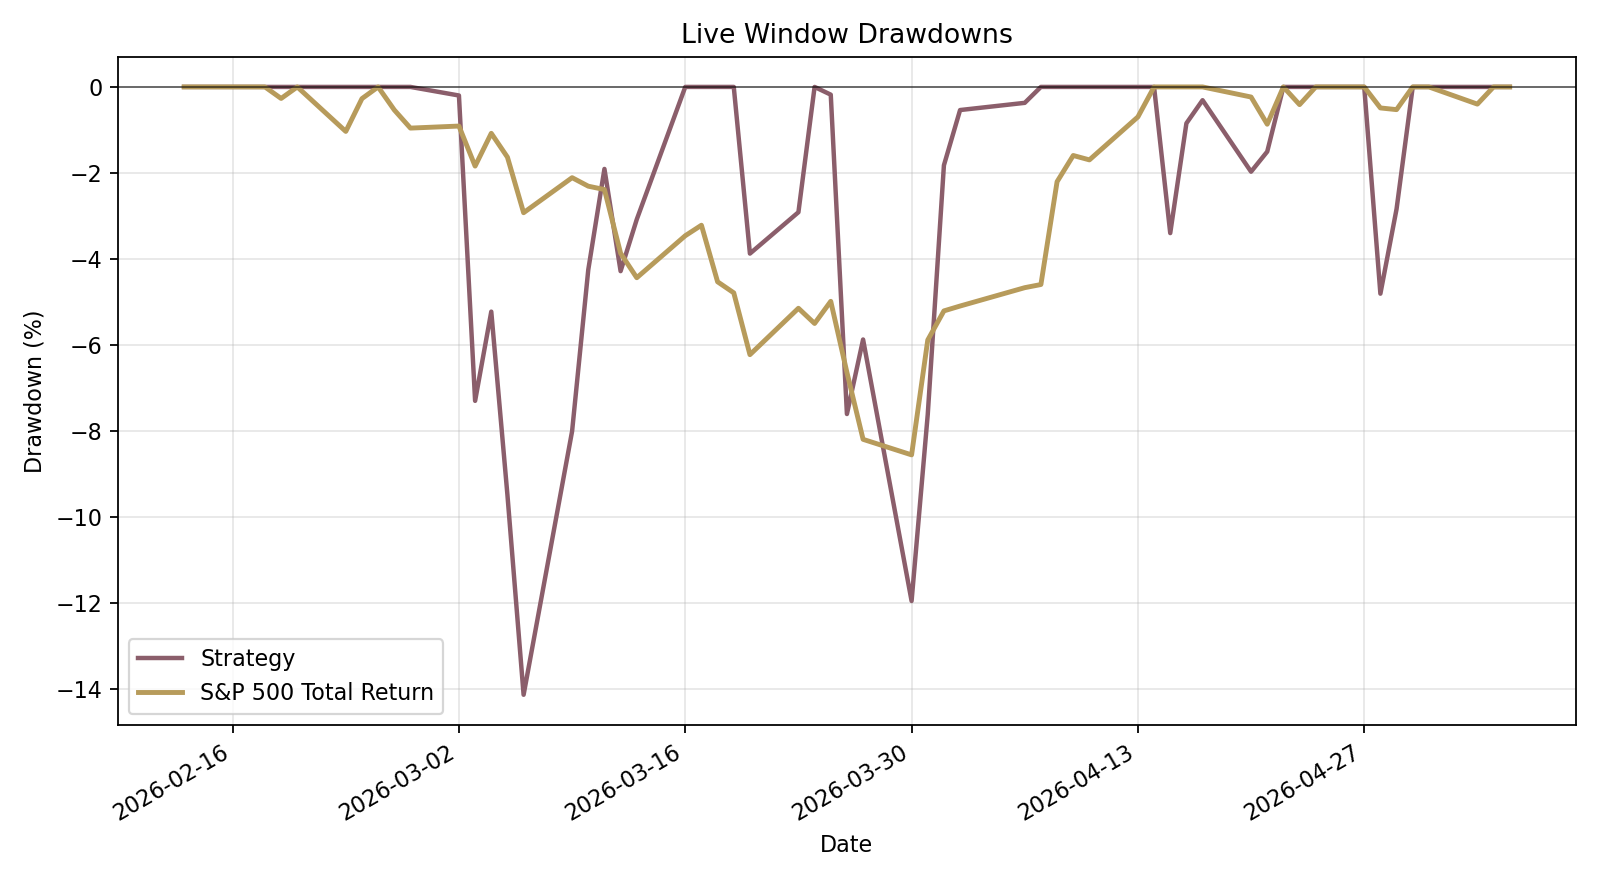
\includegraphics[width=\reportfigurewidth]{../outputs/live/strategies/momentum/figures/live_window/drawdown.png}
  \caption[Competition-window daily drawdowns]{Daily drawdowns, including the initial cash phase. Maximum drawdown
  is $-14.14\%$ for momentum and $-8.56\%$ for the benchmark.}
  \label{fig:live-drawdown}
\end{figure}

The 36 orders cost \$72 in fees and \$498.21 in spreads. Cash earned
\$931.92 and borrowing cost \$430.78. Low/base/high spread cases returned
53.86\%/53.85\%/53.84\%.

The full trade log retains decision and execution dates, identities, targets,
applied rules, rounding, suppression, constraint overrides and cash effects.
\Cref{tab:trade-excerpt} gives four entries; signals are six-month decimal
returns and prices are adjusted-unit execution references before spreads.

\begin{table}[H]
\centering
\begin{threeparttable}
\small
\begin{tabular}{@{}lllr rrr@{}}
\toprule
Date & Security & Rule & Units traded & Signal & Price (\$) & Spread (\$)\\
\midrule
2 Mar & ALB & Enter long & 593 & 1.5361 & 172.0708 & 21.12\\
2 Mar & COIN & Enter short & $-256$ & $-0.4845$ & 172.5000 & 6.64\\
1 Apr & INTC & Exit long & $-2,304$ & 0.8731 & 45.0000 & 13.95\\
1 May & LRCX & Exit long & $-451$ & 0.6002 & 254.6898 & 16.76\\
\bottomrule
\end{tabular}
\caption[Selected competition-simulation trades]{Selected competition-simulation trade-log entries.}
\label{tab:trade-excerpt}
\end{threeparttable}
\end{table}

\subsection{Attribution and reconciliation}

We apply Brinson-Fachler attribution to each sleeve, normalizing absolute
weights and reversing both stock and benchmark returns for shorts
\citep[pp.~12-14]{bacon2019}. The reconstructed benchmark total is
$\bar r^b_t=\sum_s w^b_{s,t}r^b_{s,t}$, using the same sleeve-specific signs.
For sector $s$ in interval $t$, allocation, pure selection and interaction are
\begin{equation}
 \begin{aligned}
  A_{s,t}&=(w^p_{s,t}-w^b_{s,t})(r^b_{s,t}-\bar r^b_t),\\
  S_{s,t}&=w^b_{s,t}(r^p_{s,t}-r^b_{s,t}),\qquad
  I_{s,t}=(w^p_{s,t}-w^b_{s,t})(r^p_{s,t}-r^b_{s,t}).
 \end{aligned}
\end{equation}

For an unheld sector, we set selection and interaction to zero without assigning
a realized portfolio return. Sector effects differ from raw active contributions
by $(w^p_{s,t}-w^b_{s,t})\bar r^b_t$; these adjustments cancel across normalized
sectors. Multiplying each sleeve's effects once by its positive gross exposure
expresses them relative to post-trade NAV.

\begin{figure}[H]
  \centering
  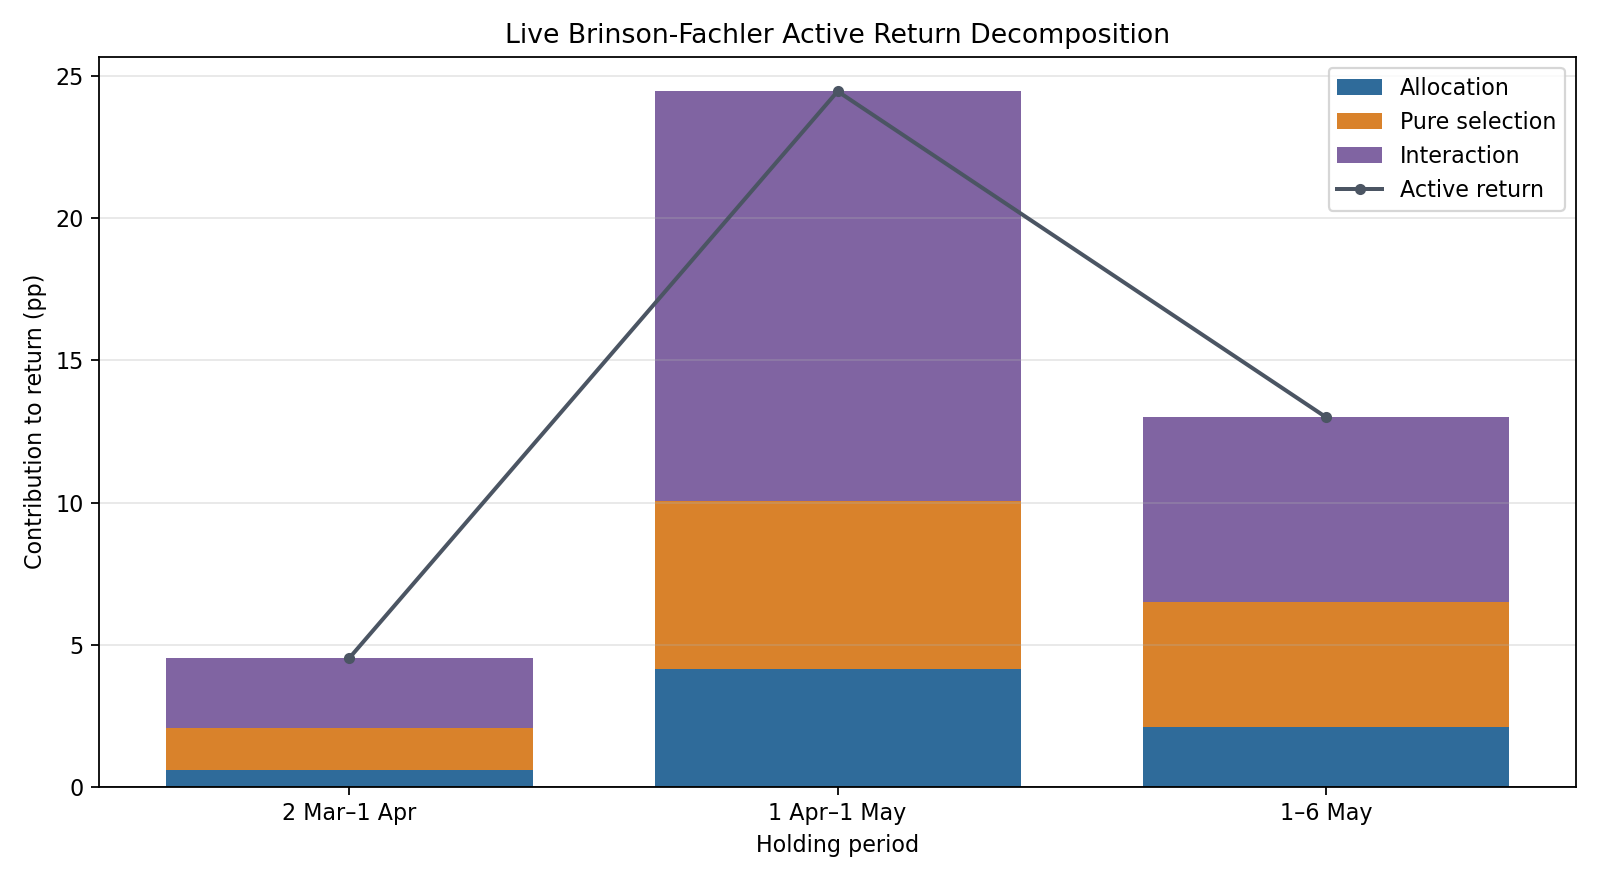
\includegraphics[width=\reportfigurewidth]{../outputs/live/strategies/momentum/figures/brinson/active_decomposition_period.png}
  \caption[Competition-window stock-sector attribution]{Brinson-Fachler allocation, pure selection and interaction over
  the three invested intervals, before account adjustments and compounding.}
  \label{fig:competition-brinson}
\end{figure}

The reconstructed benchmark covers all 503 eligible constituents in each
interval, with complete prices, shares and sectors and weights summing to one.
It returns 9.13\%, versus 8.04\% for the official index; the largest interval
gap is 1.06 percentage points (\cref{fig:benchmark-consistency}). Attribution
retains this discrepancy explicitly.

\begin{figure}[H]
  \centering
  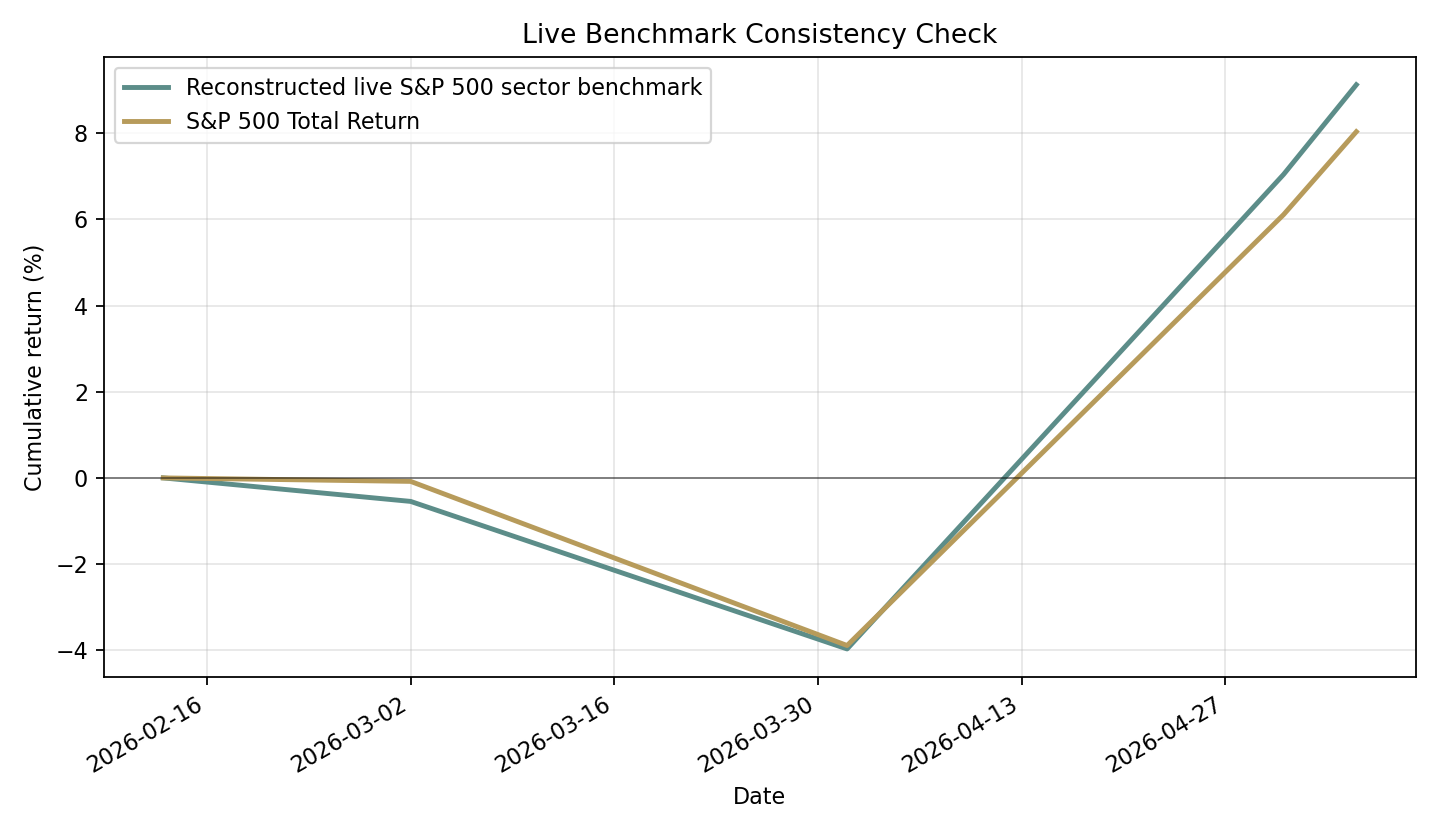
\includegraphics[width=\reportfigurewidth]{../outputs/live/strategies/momentum/figures/brinson/benchmark_consistency.png}
  \caption[Competition-window benchmark consistency]{Reconstructed sector benchmark versus the official total-return
  index, February 13 open-May 6 close, 2026. Their difference enters account attribution.}
  \label{fig:benchmark-consistency}
\end{figure}

To explain the account's net excess return, we first express all contributions
as percentages of its value at the start of each interval. We add two
adjustments to allocation, pure selection and interaction: one for our net stock exposure
differing from a 100\%-invested benchmark, and one for the gap between
reconstructed and official benchmark returns. Cash interest increases return;
borrowing, fees and spreads reduce it.

\begin{samepage}
These contributions $e_{k,t}$ sum to each interval's excess
$e_t=R^p_t-R^b_t$. Because returns compound, summing interval effects alone
does not explain cumulative excess. We multiply each by a linking factor
$L_t$: portfolio growth before interval $t$ times benchmark growth after it.
The resulting totals $E_k$ satisfy
\begin{equation}
 \begin{aligned}
 L_t&=\prod_{j<t}(1+R^p_j)\prod_{j>t}(1+R^b_j),
 \qquad E_k=\sum_t L_t e_{k,t},\\
 \sum_k E_k&=\sum_t L_t e_t=R^p_{\mathrm{cum}}-R^b_{\mathrm{cum}}.
 \end{aligned}
\end{equation}
\end{samepage}

Including the initial cash interval, the summed effects match each interval's
measured excess return to numerical precision.

\begin{table}[H]
  \centering
  \begin{threeparttable}
  \small
  \begin{tabularx}{0.82\linewidth}{@{}X S[table-format=-2.4]@{}}
    \toprule
    Linked contribution & {Percentage points} \\
    \midrule
    Sector allocation & 7.8277 \\
    Pure stock selection & 13.7421 \\
    Interaction & 26.5692 \\
    Net-exposure adjustment & -3.5176 \\
    Benchmark-reconstruction adjustment & 1.1995 \\
    Cash interest & 0.1008 \\
    Borrowing interest & -0.0455 \\
    Fixed fees & -0.0077 \\
    Spread costs & -0.0532 \\
    \midrule
    Total net account excess & 45.8152 \\
    \bottomrule
  \end{tabularx}
  \caption[Linked contributions to net account excess return]{Contributions to compounded net account excess, in percentage points. Displayed effects are rounded independently.}
  \label{tab:account-attribution}
  \end{threeparttable}
\end{table}

The chart's 42.00 percentage points simply add stock effects across invested
intervals. On a common NAV basis with compounding, the three stock effects
contribute 48.14 points. Account adjustments bring this to 45.82 points.
Interaction is the largest separate effect: 24.33 points come from the long
sleeve and 2.24 from the short sleeve. Long Information Technology alone
contributes 21.54 interaction points, reflecting its roughly 80\% sleeve weight
versus 29-31\% in the benchmark and stronger selected-stock returns, especially
in April. Pure selection contributes 13.74 points. This decomposition describes
realized concentration and relative returns; it does not establish causality
or persistent stock-picking skill.
\FloatBarrier
